% =============================================================================
%  Phone-only activity recognition in the wild:
%  a like-for-like comparison with Vaizman et al. (2017)
%
%  B.Tech Project report. Compiles with pdflatex, standard packages only:
%      cd report && pdflatex btp_report && pdflatex btp_report
%  Figures are read straight from ../outputs/figures/ (python -m asqa.figures).
% =============================================================================
\documentclass[11pt,a4paper]{article}

\usepackage[T1]{fontenc}
\usepackage[utf8]{inputenc}
\usepackage{lmodern}
\usepackage[margin=1in]{geometry}
\usepackage{graphicx}
\usepackage{booktabs}
\usepackage{amsmath}
\usepackage{microtype}
\usepackage{caption}
\usepackage{enumitem}
\usepackage{xcolor}
\usepackage{tabularx}
\usepackage{array}
\usepackage{multirow}
\usepackage{float}
\usepackage{tikz}
\usetikzlibrary{positioning,arrows.meta}
\usepackage[colorlinks=true,linkcolor=black,citecolor=black,urlcolor=blue]{hyperref}

\graphicspath{{../outputs/figures/}}
\captionsetup{font=small,labelfont=bf}
\setlist{nosep,leftmargin=1.4em}
\newcommand{\code}[1]{\texttt{\small #1}}
\newcolumntype{Y}{>{\centering\arraybackslash}X}

% --- Fill in before submission -----------------------------------------------
\newcommand{\supervisor}{Prof.\ [Supervisor name]}
\newcommand{\department}{Department of Electronics and Electrical Communication Engineering}
% -----------------------------------------------------------------------------

\title{\textbf{Phone-Only Activity Recognition in the Wild:\\
A Like-for-Like Comparison with Vaizman et al.\ (2017)}\\[6pt]
\large B.Tech Project Report}

\author{%
  P Vamshi Krishna (23EC10052)\\[2pt]
  Supervisor: \supervisor\\[2pt]
  \department\\
  Indian Institute of Technology Kharagpur%
}
\date{\today}

\begin{document}
\maketitle

\begin{abstract}
\noindent
Recognising what a person is doing from the phone in their pocket is hard in the
wild: the phone is carried in arbitrary places, recordings are intermittent, and
labels are self-reported. The ExtraSensory study of Vaizman et al.\ \cite{vaizman2017}
established the standard baseline on this problem: hand-crafted per-sensor features,
one logistic regression per label, and early or late fusion across up to six sensors.
We revisit the six body-state activities (lying down, sitting, standing, walking,
running, bicycling) with only the phone's accelerometer and gyroscope, and ask how far
a careful signal pipeline can go without the smartwatch, audio, or location. Our system
resamples both sensors onto one clock-true grid, extracts 40 interpretable features,
adds temporal context and time of day, and classifies with a hierarchical XGBoost model
followed by a time-aware HMM. To make the comparison fair we \emph{re-implement the
paper's method} and run it on exactly our users, folds, windows and labels; the
re-implementation matches the paper's published per-label balanced accuracy to within
about $0.02$. On 35 users under user-disjoint 5-fold cross-validation, our phone-only
model reaches $0.696$ accuracy and $0.566$ macro-F1, against $0.526$ / $0.366$ for the
paper's method on the same two sensors and $0.674$ / $0.478$ for its full six-sensor
system. Five further users never seen in training confirm the ordering ($0.741$ vs
$0.650$ accuracy). An ablation shows that temporal context, gradient-boosted trees, and
early fusion account for the gain, while the paper's own per-label metric still favours
its six-sensor system ($0.776$ vs $0.744$), for reasons we explain.
\end{abstract}

% =============================================================================
\section{Introduction}
% =============================================================================

Automatic recognition of a person's behavioural context supports health monitoring,
ageing care, and just-in-time interventions \cite{vaizman2017}. Most early systems were
validated under controlled conditions: scripted activities, a fixed device position,
and a researcher watching. Vaizman et al.\ argued that such results do not transfer to
real life and collected the ExtraSensory dataset \emph{in the wild}: 60 people used their
own phones, carried them however they liked, and self-reported their context over about
a week. Their baseline---per-sensor features, logistic regression, and three fusion
strategies over six sensors---remains the reference point for this dataset.

Two observations motivate this project. First, the paper's strongest results rely on a
smartwatch, audio and location, which many deployments cannot assume; the phone's own
motion sensors are the one modality that is always there. Second, the paper treats every
minute independently and uses a linear classifier, leaving two obvious levers untested:
the temporal structure of behaviour, and non-linear models. This report asks a narrow
question and answers it under a strict protocol:

\begin{quote}
\emph{Using only the phone's accelerometer and gyroscope, how does a carefully engineered
recogniser compare with the paper's method on the same data---and which design choices
are responsible for the difference?}
\end{quote}

\paragraph{Contributions.}
\begin{enumerate}
\item A faithful \textbf{re-implementation of the paper's baseline} (features, per-label
logistic regression with its C search, EF/LFA/LFL fusion), run on our exact users, folds,
windows and labels, and checked against the published numbers (\S\ref{sec:repro}).
\item A \textbf{phone-only recogniser} built on clock-true resampling, 40 interpretable
features, temporal context, time of day, label cleaning, hierarchical XGBoost and a
time-aware HMM (\S\ref{sec:method}).
\item A \textbf{like-for-like comparison} on cross-validation and on five held-out users,
reported on multiclass metrics and on the paper's own per-label metric
(\S\ref{sec:results}).
\item An \textbf{ablation} that separates the components that consistently help from
those that sit within fold-to-fold noise (\S\ref{sec:ablation}).
\end{enumerate}

The recogniser also drives a grounded question-answering demo with a small language
model; it is described briefly in \S\ref{sec:demo}, but its scores are not part of the
comparison.

% =============================================================================
\section{The reference study}
\label{sec:paper}
% =============================================================================

\paragraph{Data.}
ExtraSensory \cite{vaizman2017} records a 20-second burst of sensor data every minute
from each participant's phone and an optional Pebble watch. Participants labelled their
context through an app offering over 100 labels, any combination of which may apply to a
minute. The public release contains 308{,}320 labelled minutes from 60 users, the raw
signals, and pre-computed features for each sensor.

\paragraph{Method.}
For every sensor $s$ the paper computes a fixed feature vector: 26 magnitude, spectral
and autocorrelation statistics for the phone accelerometer (Acc) and gyroscope (Gyro),
46 for the watch accelerometer (WAcc), 17 relative-location features (Loc), 26 MFCC
statistics (Aud) and 34 phone-state indicators including time of day (PS). Each label is
modelled \emph{independently} by a binary logistic regression with balanced class
weights; the regularisation constant $C$ is chosen from $\{10^{-3},\dots,10^{2}\}$ by F1
on a random third of the training data. Sensors are combined in three ways:
\begin{itemize}
\item \textbf{EF} (early fusion): concatenate the standardised features of all sensors;
\item \textbf{LFA} (late fusion, average): average the per-sensor probabilities;
\item \textbf{LFL} (late fusion, learned): a second logistic regression over them.
\end{itemize}

\paragraph{Evaluation.}
The paper reports, per label, the \emph{balanced accuracy} (BA) of that label's yes/no
decision, $\mathrm{BA}=\tfrac12(\mathrm{TPR}+\mathrm{TNR})$, under user-disjoint 5-fold
cross-validation. For the body-state labels it also shows multiclass confusion matrices
(its Fig.~4B--C), whose diagonals give per-class recall. With phone Acc+Gyro the
diagonal for lying, sitting, walking, running and bicycling is $0.79, 0.44, 0.51, 0.19,
0.50$ (mean $0.49$); adding the watch raises it to $0.82, 0.67, 0.56, 0.23, 0.66$ (mean
$0.59$).

The two views measure different things. A per-label detector is free to say ``yes'' to
several labels at once, and each label is scored against its own threshold. A
recogniser that must name \emph{one} activity per window is scored on whether that
single choice is right. We report both, because a method tuned for one view does not
automatically win the other.

% =============================================================================
\section{Data and protocol}
\label{sec:data}
% =============================================================================

\paragraph{Users and windows.}
We use a working set of 35 ExtraSensory users with raw phone accelerometer and gyroscope
recordings, plus five further users kept aside as a held-out set. A window is
the 15-second span (375 samples at 25\,Hz) of a minute's recording in which both sensors
were observing; windows with a sensor gap wider than $0.5$\,s are rejected rather than
interpolated. This leaves \textbf{165{,}787 labelled windows} for cross-validation and
31{,}557 for the held-out users.

\paragraph{Labels.}
We use six body-state labels, taking the dataset's corrected columns where they exist
(\code{LYING\_DOWN}, \code{SITTING}, \code{OR\_standing}, \code{FIX\_walking},
\code{FIX\_running}, \code{BICYCLING}). A window is kept only when exactly one of the six
is active, so every window has a single true class. Table~\ref{tab:classes} shows the
resulting imbalance: running is $0.34\%$ of windows, sitting $44\%$.

\begin{table}[H]
\centering\small
\caption{Labelled windows per class.}
\label{tab:classes}
\begin{tabular}{@{}lrrrrrr|r@{}}
\toprule
& Lying & Sitting & Standing & Walking & Running & Bicycling & Total \\
\midrule
Cross-validation (35 users) & 55{,}789 & 73{,}301 & 20{,}748 & 11{,}975 & 567 & 3{,}407 & 165{,}787 \\
Held-out (5 users)          & 12{,}236 & 13{,}239 &  2{,}837 &  2{,}680 &  58 &   160 &  31{,}557 \\
\bottomrule
\end{tabular}
\end{table}

\paragraph{Folds.}
Windows from one person are strongly correlated, so a random split would put the same
person in training and test and inflate every score. All experiments use the same
\textbf{user-disjoint 5-fold} assignment, built so that the users carrying the rare
classes are spread across folds. Within a fold, our model trains on the training users,
tunes early stopping and calibration on a small set of validation users, and is scored on
the test users. The paper's method trains on training $\cup$ validation users, so both
sides see exactly the same people.

\paragraph{Same windows, same labels.}
The paper's pre-computed features are indexed by minute; we look up the row for each of
our windows, so both methods are scored on the \emph{identical} 165{,}787 windows with
the identical labels. Every test label is raw: label cleaning (\S\ref{sec:cleaning})
touches training data only.

\paragraph{Metrics.}
We report \textbf{accuracy}; \textbf{balanced accuracy}, the mean per-class recall,
which is chance-corrected for imbalance; \textbf{macro-F1}, which also penalises false
alarms on rare classes; and the paper's \textbf{per-label binary BA}. Values are
mean~$\pm$~standard deviation over the five folds.

% =============================================================================
\section{Our recogniser}
\label{sec:method}
% =============================================================================

Figure~\ref{fig:pipeline} shows the pipeline. Each stage adds one structure to the
previous one, and every stage is a separate module with its own tests.

\begin{figure}[H]
\centering
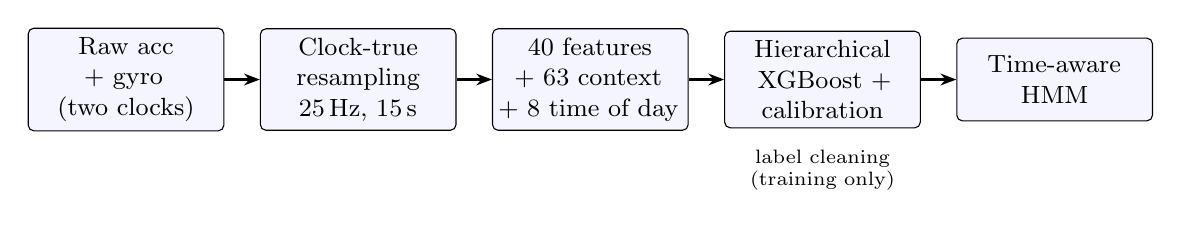
\begin{tikzpicture}[
  box/.style={draw, rounded corners=2pt, align=center, font=\small,
              minimum height=1.05cm, text width=2.25cm, fill=blue!4},
  arr/.style={-{Stealth[length=2mm]}, thick}]
\node[box] (a) {Raw acc + gyro\\(two clocks)};
\node[box, right=0.45cm of a] (b) {Clock-true\\resampling\\25\,Hz, 15\,s};
\node[box, right=0.45cm of b] (c) {40 features\\+ 63 context\\+ 8 time of day};
\node[box, right=0.45cm of c] (d) {Hierarchical\\XGBoost +\\calibration};
\node[box, right=0.45cm of d] (e) {Time-aware\\HMM};
\draw[arr] (a) -- (b);
\draw[arr] (b) -- (c);
\draw[arr] (c) -- (d);
\draw[arr] (d) -- (e);
\node[font=\scriptsize, below=0.15cm of d, text width=2.6cm, align=center] {label cleaning\\(training only)};
\end{tikzpicture}
\caption{Recognition pipeline. Label cleaning removes training windows whose labels the
signal cannot support; test labels are never modified.}
\label{fig:pipeline}
\end{figure}

\subsection{Clock-true resampling}
ExtraSensory's accelerometer and gyroscope run on independent, skewed clocks; measured
inter-sample intervals range from $0.024$\,s to $0.077$\,s. Windowing by sample index
therefore stretches time differently for each user (a $2.0$\,Hz walking cadence reads as
$2.3$\,Hz), and pairing the two sensors by index misaligns them by a growing offset. We
interpolate both streams onto one absolute grid at exactly $0.04$\,s per sample, over the
interval both sensors observed. A window with a gap wider than $0.5$\,s is rejected with
a recorded reason instead of being bridged by a straight line.

\subsection{Features}
\paragraph{Per-window (40).} A $0.3$\,Hz low-pass filter splits acceleration into
gravity, which gives device tilt (what separates lying from upright), and body
acceleration, which gives motion energy. Autocorrelation recovers cadence; the rest are
spectral entropy, four band powers, jerk, crest factor, zero-crossing rate, gyroscope
magnitude and axis dominance, and the accelerometer--gyroscope correlation. Every
feature has a physical meaning, so an explanation can cite it.

\paragraph{Temporal context (63).} A single still window cannot tell lying from sitting
when the phone is on a table; its neighbours often can. For five base channels (motion
energy, tilt, cadence, rotation, spectral entropy) we add rolling means and standard
deviations over $\pm2$, $\pm5$, $\pm15$ and $\pm30$ windows, the previous and next values
and their differences, plus the gaps to the neighbours and the number of windows within
30 minutes. Neighbours more than 40 minutes away are ignored, because adjacent rows of an
intermittent recording can be hours apart.

\paragraph{Time of day (8).} Following the paper's own encoding, each window's local
(San Diego) hour switches on two of eight half-overlapping six-hour bins. This is the
one phone-state cue we adopt; it costs nothing to compute from the timestamp.

\subsection{Label cleaning}
\label{sec:cleaning}
The dataset's \code{FIX\_walking} and \code{FIX\_running} columns already contain the
paper's rule-based corrections; we verified that no walking or running window co-occurs
with a vehicle label. What remains are windows labelled walking, running or bicycling
whose signal shows no motion at all---the phone was on a table or in a still bag, so no
phone-only model can see the activity. We drop such windows from \emph{training and
validation} when their body-acceleration energy is at or below the 90th percentile of
training lying-down windows ($\approx0.008$\,g, fitted per fold). This removes about 17\%
of walking, 25\% of running and 11\% of bicycling training windows.

\subsection{Hierarchical XGBoost}
A first gradient-boosted model \cite{xgboost} separates static (lying, sitting, standing) from dynamic
(walking, running, bicycling) windows; two further models choose the class within each
branch. Leaf probabilities combine as
$P(\text{leaf}) = P(\text{branch})\,P(\text{leaf}\mid\text{branch})$, are renormalised,
and are calibrated by one temperature fitted on the validation users ($0.93$--$1.33$
across folds). Inverse-frequency sample weights keep the rare classes from being
ignored. Trees suit these features: the context columns are highly correlated, the units
differ by orders of magnitude, and the useful decisions are interactions (high tilt
\emph{and} low energy).

\subsection{Time-aware HMM}
Independent per-window decisions flicker. An HMM over each recording uses the calibrated
probabilities as emissions and a transition matrix estimated from training sequences. Because
windows are irregularly spaced, the per-minute transition matrix is raised to the power
$\Delta t/60$, so after a long gap the state distribution relaxes towards the stationary
one instead of assuming the activity continued. The demo decodes with Viterbi; we report
posterior decoding alongside it.

% =============================================================================
\section{Reproducing the reference method}
\label{sec:repro}
% =============================================================================

We re-implemented the paper's pipeline exactly as described in its supplement: the
published per-sensor features (whose sizes match the paper: 26, 26, 46, 17, 26 and 34),
per-sensor standardisation with training statistics, one binary logistic regression per
label with balanced class weights and the F1-driven $C$ search, and EF, LFA and LFL
fusion. Missing sensors (the watch is absent for 35\% of our windows) are handled as
the paper's design implies: zero after standardisation for EF, single-sensor models
trained only where their sensor exists, LFA averaging the sensors present, and a neutral
$0.5$ for an absent sensor in LFL. For multiclass scoring, a window's prediction is the
label with the highest probability.

Table~\ref{tab:repro} compares the reproduction's per-label binary BA with the paper's
published values. Nearly every cell agrees within $0.02$, despite our using 35 of the 60
users; the largest gap is bicycling under fusion ($0.03$--$0.04$). We therefore treat the
reproduction as a fair stand-in for the published system.

\begin{table}[H]
\centering\small
\caption{Faithfulness check: per-label binary balanced accuracy, reproduction / published
(Table S1 of \cite{vaizman2017}).}
\label{tab:repro}
\begin{tabular}{@{}lcccccc@{}}
\toprule
System & Lying & Sitting & Standing & Walking & Running & Bicycling \\
\midrule
Acc only        & 0.73 / 0.72 & 0.62 / 0.63 & 0.60 / 0.60 & 0.76 / 0.77 & 0.71 / 0.69 & 0.81 / 0.81 \\
Gyro only       & 0.69 / 0.69 & 0.60 / 0.61 & 0.60 / 0.59 & 0.78 / 0.80 & 0.76 / 0.66 & 0.80 / 0.81 \\
EF, 6 sensors   & 0.87 / 0.87 & 0.77 / 0.76 & 0.66 / 0.68 & 0.79 / 0.80 & 0.64 / 0.62 & 0.83 / 0.87 \\
LFA, 6 sensors  & 0.87 / 0.86 & 0.76 / 0.75 & 0.65 / 0.67 & 0.79 / 0.80 & 0.75 / 0.69 & 0.83 / 0.87 \\
LFL, 6 sensors  & 0.88 / 0.88 & 0.77 / 0.75 & 0.66 / 0.68 & 0.80 / 0.80 & 0.71 / 0.71 & 0.84 / 0.87 \\
\bottomrule
\end{tabular}
\end{table}

% =============================================================================
\section{Results}
\label{sec:results}
% =============================================================================

\subsection{Main comparison}

Table~\ref{tab:main} is the central result. With the \emph{same two phone sensors}, our
recogniser beats every fusion variant of the paper's method on every metric; even
without temporal context it already leads on macro-F1 ($0.433$ vs $0.366$ at best). With
context it also exceeds the paper's full six-sensor system---watch, audio, location and
phone state included---by $+0.022$ accuracy, $+0.034$ balanced accuracy and $+0.088$
macro-F1.

\begin{table}[H]
\centering\small
\caption{User-disjoint 5-fold cross-validation, identical test windows and raw labels
(mean $\pm$ std over folds). Best per column in bold.}
\label{tab:main}
\begin{tabularx}{\textwidth}{@{}l l YYY@{}}
\toprule
System & Sensors & Accuracy & Balanced acc. & Macro-F1 \\
\midrule
Paper, EF  & phone Acc+Gyro & $0.479\pm0.043$ & $0.437\pm0.051$ & $0.348\pm0.018$ \\
Paper, LFA & phone Acc+Gyro & $0.526\pm0.012$ & $0.401\pm0.021$ & $0.366\pm0.020$ \\
Paper, LFL & phone Acc+Gyro & $0.505\pm0.015$ & $0.441\pm0.066$ & $0.330\pm0.023$ \\
\addlinespace
Paper, EF  & all six        & $0.662\pm0.040$ & $0.527\pm0.056$ & $0.467\pm0.023$ \\
Paper, LFA & all six        & $0.674\pm0.034$ & $0.502\pm0.039$ & $0.478\pm0.030$ \\
Paper, LFL & all six        & $0.673\pm0.046$ & $0.523\pm0.059$ & $0.468\pm0.023$ \\
\midrule
Ours, no context            & phone Acc+Gyro & $0.528\pm0.038$ & $0.461\pm0.058$ & $0.433\pm0.058$ \\
Ours, full (per window)     & phone Acc+Gyro & $0.696\pm0.037$ & $0.561\pm0.071$ & $0.566\pm0.076$ \\
Ours + HMM, Viterbi (demo)  & phone Acc+Gyro & $\mathbf{0.718\pm0.037}$ & $0.555\pm0.079$ & $0.564\pm0.078$ \\
Ours + HMM, posterior       & phone Acc+Gyro & $0.716\pm0.037$ & $\mathbf{0.569\pm0.077}$ & $\mathbf{0.583\pm0.078}$ \\
\bottomrule
\end{tabularx}
\end{table}

\subsection{Where the gain comes from, class by class}

Figures~\ref{fig:confusion} and~\ref{fig:recall} break the comparison down by class on
the identical windows. Lying down is easy for everyone (recall $0.82$--$0.87$): tilt
alone identifies it. The differences are in the classes that look alike in a single
window. Sitting and standing are both still and upright; the paper's phone-only method
recalls them at $0.43$ and $0.15$, and confuses $42\%$ of sitting with lying. Temporal
context and time of day lift sitting to $0.73$ and standing to $0.32$, above even the
six-sensor system ($0.68$, $0.25$). Walking rises from $0.44$ (phone) and $0.50$ (six
sensors) to $0.64$. Bicycling is the one class where the watch and location help the
paper more than context helps us ($0.62$ vs $0.58$).

Running is the hardest class for all three systems. The paper's method, reduced to one
choice per window, almost never names it ($0.01$ and $0.06$ recall); ours reaches $0.18$,
and more than half of the misses are read as walking, which shares its rhythm. Part of
the ceiling is in the labels themselves: a quarter of running-labelled windows carry no
more motion than lying down.

\begin{figure}[H]
\centering
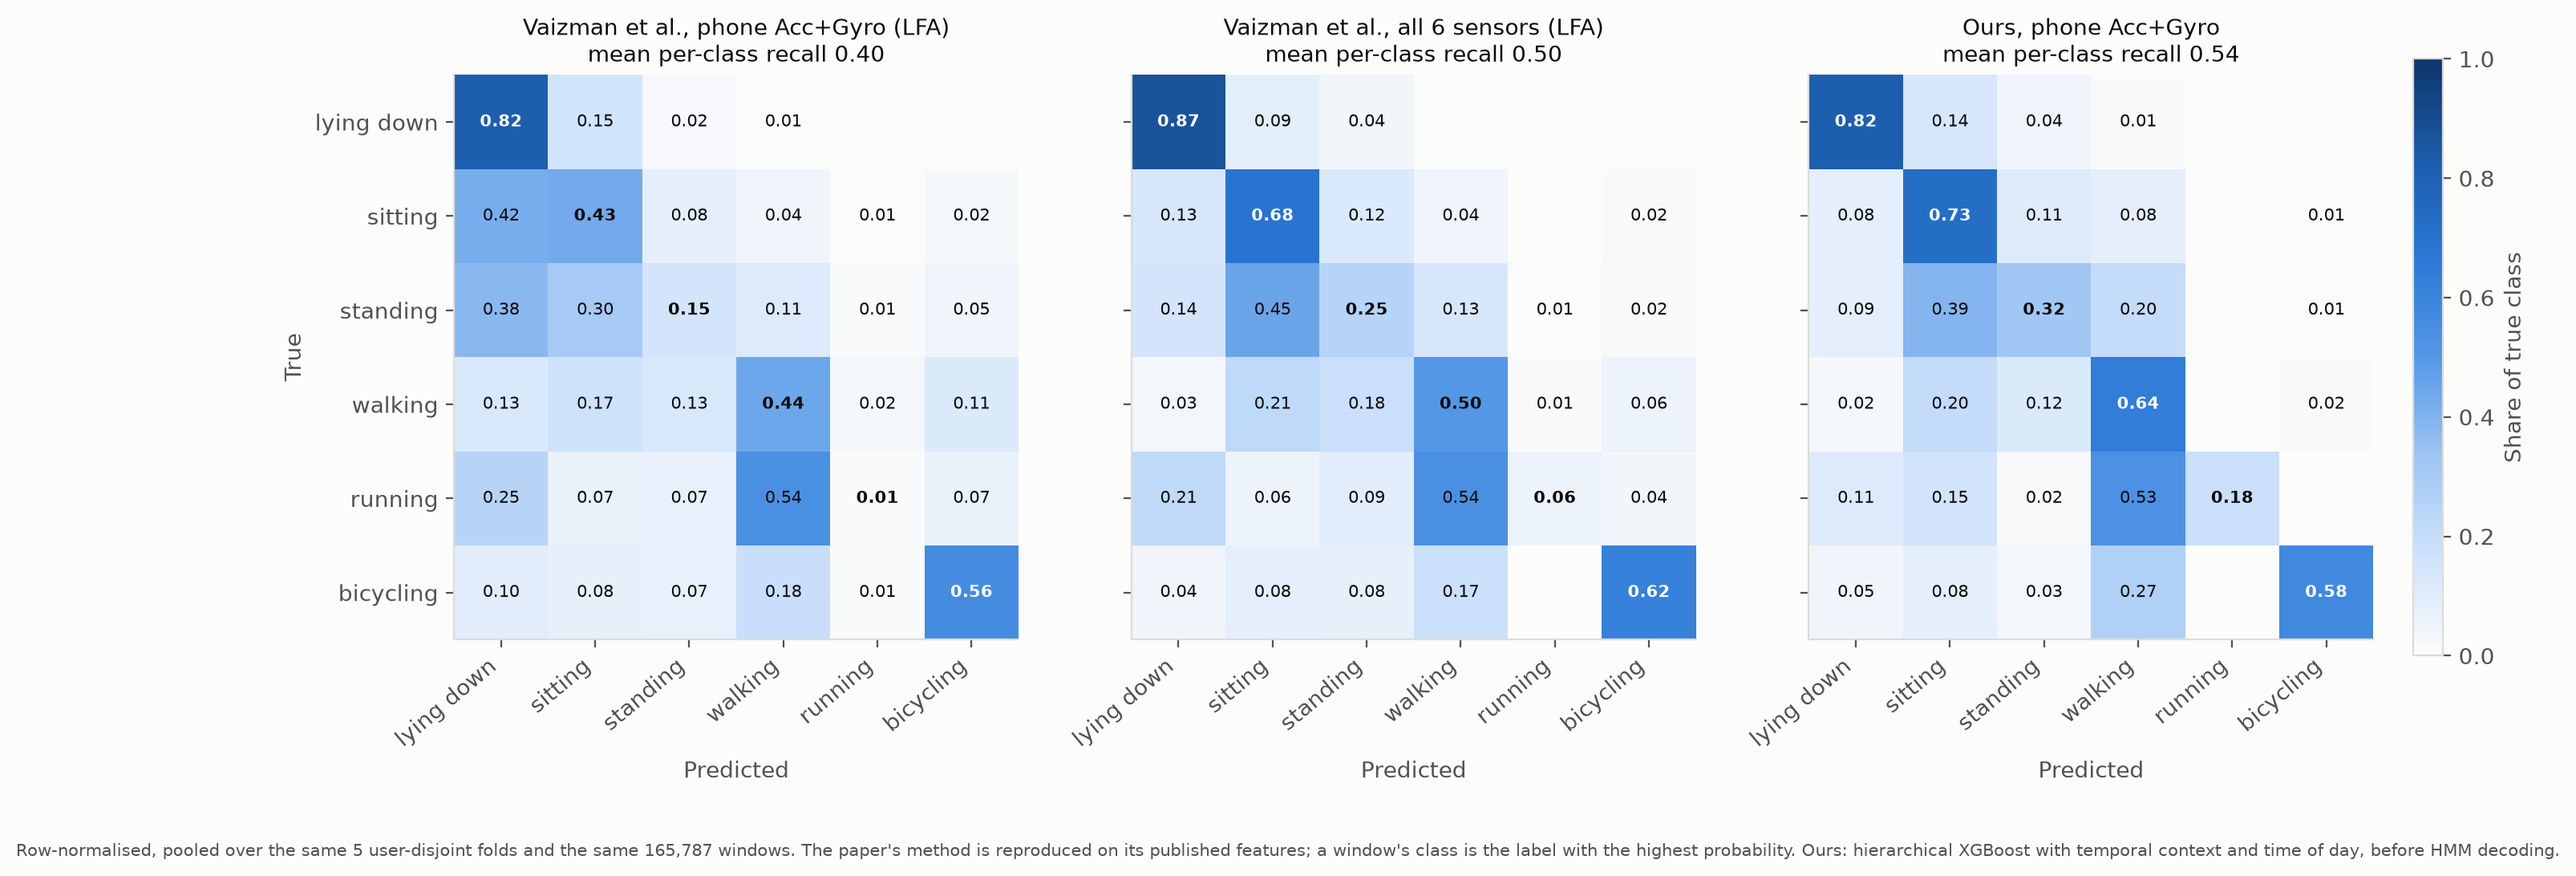
\includegraphics[width=\textwidth]{fig6_paper_vs_ours_confusion.png}
\caption{Row-normalised confusion matrices on the same 165{,}787 windows: the paper's
method with phone sensors (left) and with all six sensors (centre), and ours with phone
sensors (right). Diagonal values are per-class recall.}
\label{fig:confusion}
\end{figure}

\begin{figure}[H]
\centering
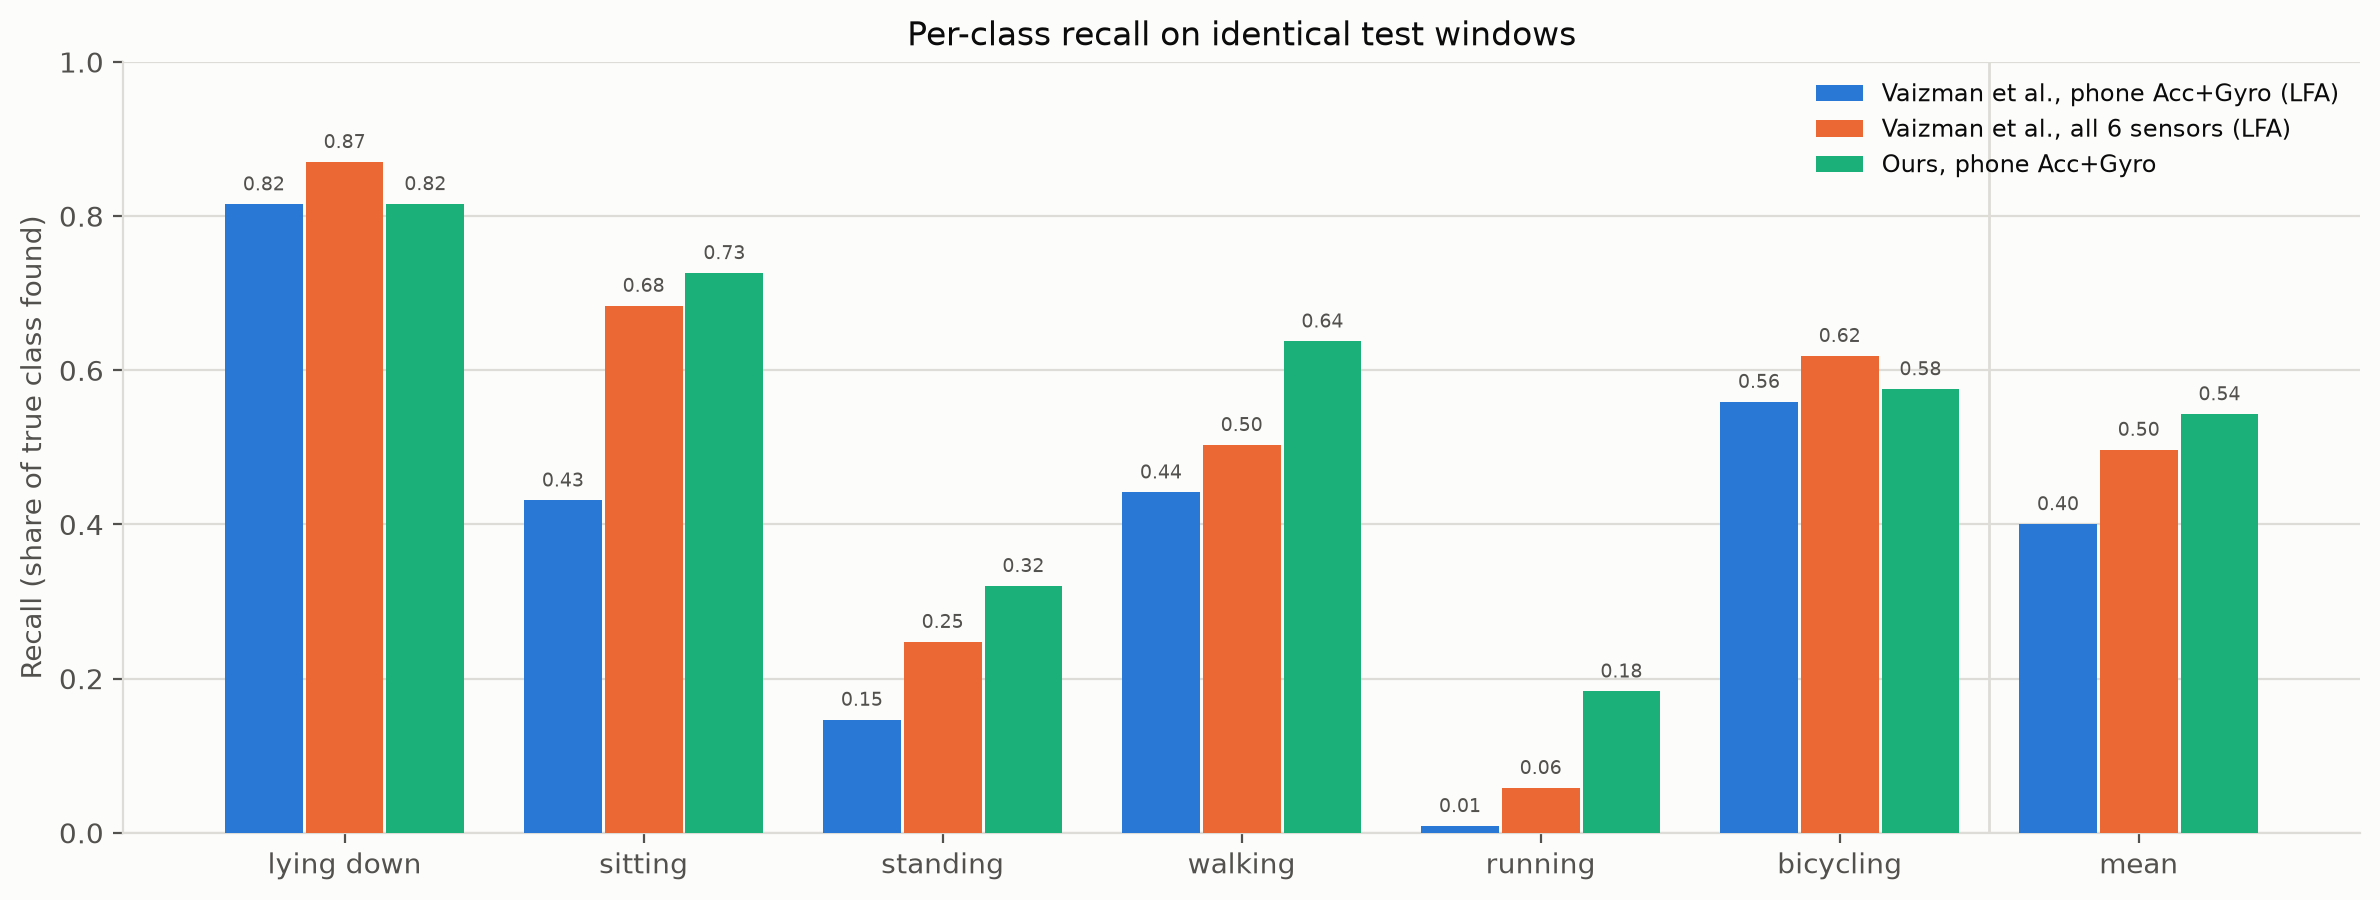
\includegraphics[width=0.92\textwidth]{fig7_per_class_recall.png}
\caption{Per-class recall for the three systems of Fig.~\ref{fig:confusion}. Every bar
carries its value; the right-hand group is the mean (balanced accuracy, pooled).}
\label{fig:recall}
\end{figure}

\subsection{On the paper's own metric}

Table~\ref{tab:binary} scores all systems the paper's way: each label's yes/no decision,
by balanced accuracy. Here the picture is mixed. Ours still beats the paper's phone-only
method ($0.744$ vs $0.720$), but the six-sensor system leads ($0.776$), with the gap in
running, bicycling and standing.

\begin{table}[H]
\centering\small
\caption{Per-label binary balanced accuracy, mean over folds.}
\label{tab:binary}
\begin{tabular}{@{}lccccccc@{}}
\toprule
System & Lying & Sitting & Standing & Walking & Running & Bicycling & Mean \\
\midrule
Paper LFA, phone Acc+Gyro & 0.73 & 0.63 & 0.60 & 0.78 & 0.76 & 0.83 & 0.720 \\
Paper LFA, all six        & 0.87 & 0.76 & 0.65 & 0.79 & 0.75 & 0.83 & \textbf{0.776} \\
Ours, no context          & 0.70 & 0.65 & 0.52 & 0.77 & 0.62 & 0.78 & 0.674 \\
Ours, full                & 0.87 & 0.76 & 0.62 & 0.78 & 0.65 & 0.78 & 0.744 \\
\bottomrule
\end{tabular}
\end{table}

The difference is structural, not a hidden weakness. The paper trains an independent
detector per label, each with balanced weights and its own $0.5$ threshold, so a rare
label can fire whenever its own evidence is moderately strong---even if another label is
far more likely. That maximises per-label BA but, when the same detectors must name one
activity, rare classes almost never win (running recall $0.01$--$0.06$ in
Fig.~\ref{fig:recall}). Our model makes the single choice directly, which is what a
six-way recogniser is for, and it is why ours wins every multiclass metric in
Table~\ref{tab:main}.

\subsection{Held-out users}

Five users were never used to train, tune, or select anything. Each fold's saved model
is scored on them, and the paper's method is trained on that same fold's users, so both
sides see identical training data (Table~\ref{tab:holdout}). The ordering is unchanged:
ours leads the paper's phone-only method by $+0.17$ accuracy and $+0.15$ macro-F1, and its
six-sensor method by $+0.09$ and $+0.09$. Balanced accuracy is close to the six-sensor
system here, but with only 58 running and 160 bicycling windows those two classes are
noisy.

\begin{table}[H]
\centering\small
\caption{Five held-out users (31{,}557 windows), mean $\pm$ std over the five fold models.}
\label{tab:holdout}
\begin{tabularx}{\textwidth}{@{}l YYY@{}}
\toprule
System & Accuracy & Balanced acc. & Macro-F1 \\
\midrule
Paper, best phone-only (LFA)   & $0.571\pm0.006$ & $0.428\pm0.005$ & $0.349\pm0.005$ \\
Paper, best six-sensor (LFA)   & $0.650\pm0.012$ & $0.491\pm0.014$ & $0.409\pm0.005$ \\
Paper, six-sensor (EF)         & $0.633\pm0.016$ & $0.510\pm0.027$ & $0.388\pm0.011$ \\
\midrule
Ours, per window               & $0.713\pm0.007$ & $0.515\pm0.010$ & $0.478\pm0.018$ \\
Ours + HMM, Viterbi            & $\mathbf{0.741\pm0.006}$ & $0.518\pm0.010$ & $\mathbf{0.496\pm0.017}$ \\
Ours + HMM, posterior          & $0.740\pm0.006$ & $\mathbf{0.519\pm0.011}$ & $\mathbf{0.496\pm0.017}$ \\
\bottomrule
\end{tabularx}
\end{table}

\subsection{Ablation}
\label{sec:ablation}

Each row of Fig.~\ref{fig:ablation} changes one thing relative to the deployed
per-window model and is scored on the same folds. Because fold-to-fold variation is large
(std $\approx0.07$), we judge each change by \emph{paired} differences: how much the
deployed model wins by, and in how many of the five folds (Table~\ref{tab:ablation}).

\begin{figure}[H]
\centering
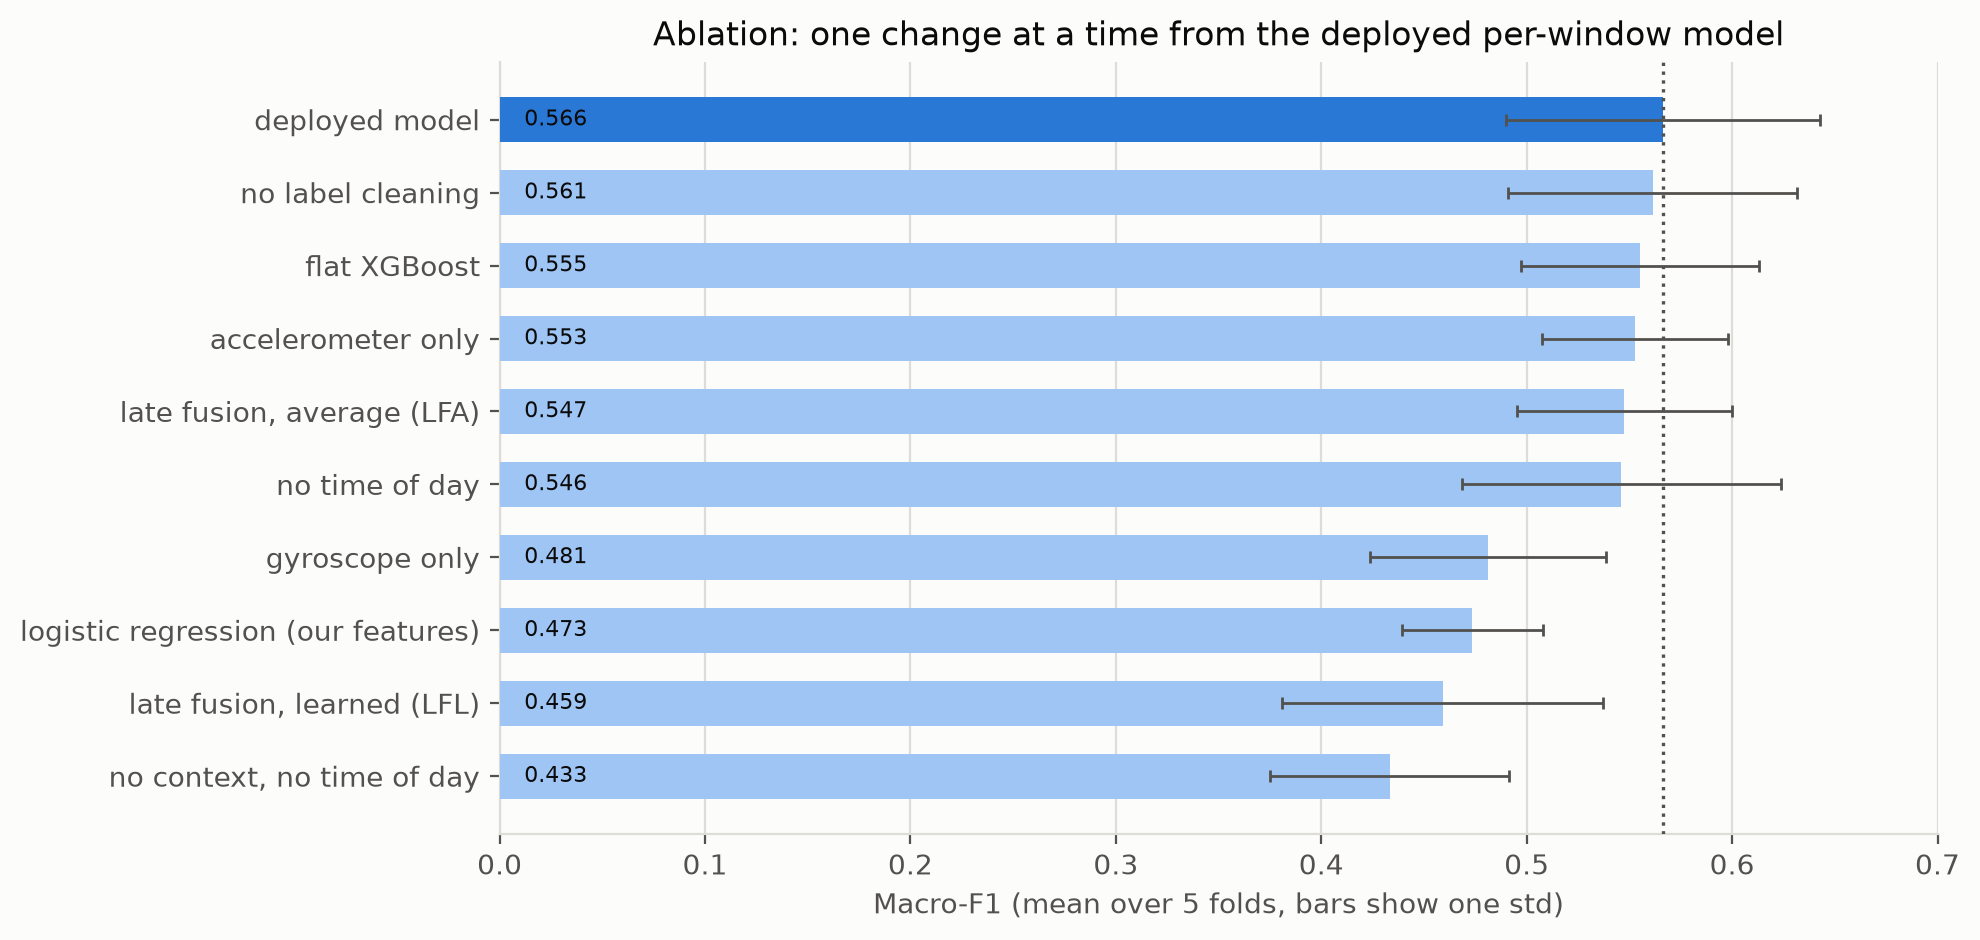
\includegraphics[width=0.8\textwidth]{fig8_ablation.png}
\caption{Macro-F1 of each ablation (mean over folds; whiskers one std). The dotted line
is the deployed model.}
\label{fig:ablation}
\end{figure}

\begin{table}[H]
\centering\small
\caption{Paired ablation: deployed minus variant, macro-F1, with the number of folds in
which the deployed model is better.}
\label{tab:ablation}
\begin{tabular}{@{}lccc@{}}
\toprule
Variant & Macro-F1 & Deployed better by & Folds \\
\midrule
No temporal context, no time of day   & 0.433 & $+0.133$ & 5/5 \\
Learned late fusion (LFL)             & 0.459 & $+0.107$ & 5/5 \\
Logistic regression (our features)    & 0.473 & $+0.093$ & 5/5 \\
Gyroscope only                        & 0.481 & $+0.085$ & 5/5 \\
No time of day                        & 0.546 & $+0.020$ & 5/5 \\
\addlinespace
Average late fusion (LFA)             & 0.547 & $+0.019$ & 2/5 \\
Accelerometer only                    & 0.553 & $+0.014$ & 2/5 \\
Flat XGBoost (no hierarchy)           & 0.555 & $+0.011$ & 2/5 \\
No label cleaning                     & 0.561 & $+0.005$ & 4/5 \\
\bottomrule
\end{tabular}
\end{table}

Four findings are consistent in every fold. \textbf{Temporal context} is the largest single
gain. \textbf{Gradient-boosted trees} beat logistic regression on the same 111 features
by $0.09$ macro-F1, so the paper's linear classifier is a real limitation, not only its
features. \textbf{Early fusion} beats learned late fusion: concatenating acc and gyro lets
one model use their interactions, such as their correlation, which per-sensor models
cannot. \textbf{Time of day} helps modestly but reliably. The other changes sit within
noise: the static/dynamic hierarchy, label cleaning, and fusing the gyroscope at all on
top of the accelerometer. We keep them because they do not hurt and the hierarchy gives
better balanced accuracy, but we do not claim them as gains.

\paragraph{Decoding.} Posterior decoding improves every metric over per-window prediction
(macro-F1 better in 5/5 folds); Viterbi raises accuracy by $+0.023$ but leaves balanced
accuracy and macro-F1 flat. On the held-out users the two are tied. The demo keeps
Viterbi because it needs one coherent path to form activity bouts; for recognition
scores, posterior decoding is the better choice.

\subsection{Development log}

Table~\ref{tab:phases} records how the system reached its final form. The starting point
was a seven-class system built for a course challenge, which split ExtraSensory's single
standing label into ``in place'' and ``moving'' with an energy threshold. That derived
class was the weakest (F1 $0.227$) and was not supported by any annotation, so we dropped
it.

\begin{table}[H]
\centering\small
\caption{Per-window results with context after each change (5-fold CV, raw test labels).}
\label{tab:phases}
\begin{tabular}{@{}lccc@{}}
\toprule
Stage & Accuracy & Balanced acc. & Macro-F1 \\
\midrule
Challenge system, 7 classes incl.\ derived standing split & 0.660 & -- & 0.529 \\
6 annotated classes                    & 0.665 & 0.557 & 0.551 \\
$+$ time of day                        & 0.695 & 0.564 & 0.561 \\
$+$ label cleaning (final)             & 0.696 & 0.561 & 0.566 \\
\bottomrule
\end{tabular}
\end{table}

% =============================================================================
\section{Robustness, cost, and the question-answering demo}
\label{sec:demo}
% =============================================================================

\paragraph{Robustness.}
Degrading the raw 25\,Hz signal of two held-out users (4{,}977 windows) before feature
extraction shows graceful decline (Fig.~\ref{fig:robust}): accelerometer noise of
$\sigma=0.2$\,g lowers decoded accuracy from $0.809$ to $0.619$; losing half the samples
barely matters ($0.804$), which is what clock-true resampling is designed to absorb; and
reducing the sampling rate to 5\,Hz costs four points ($0.767$).

\begin{figure}[H]
\centering
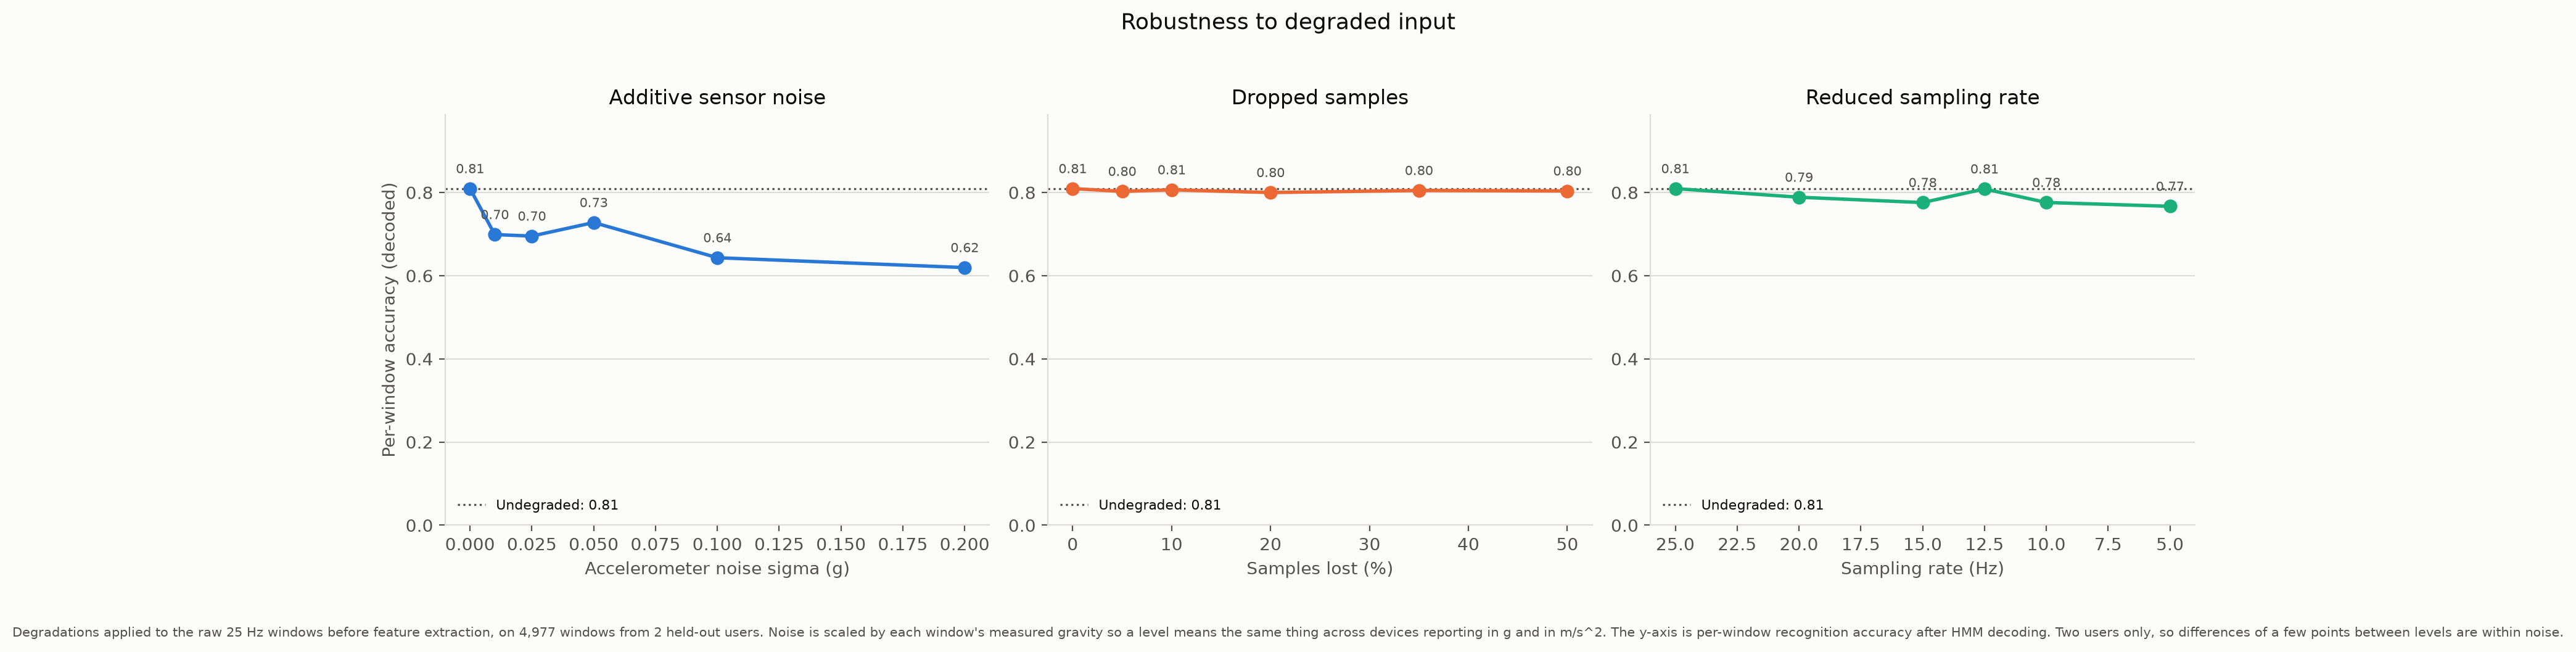
\includegraphics[width=\textwidth]{fig5_robustness.png}
\caption{Decoded per-window accuracy under additive noise, sample dropout and reduced
sampling rate (two held-out users; differences of a few points are within noise).}
\label{fig:robust}
\end{figure}

\paragraph{Cost.}
On a laptop CPU the deployed model is 4.7\,MB and classifies a window in $0.45$\,ms, plus
$0.34$\,ms of feature extraction. A depth-3, 100-tree variant fits in $0.85$\,MB at
$0.606$ instead of $0.643$ accuracy on the same fold, a candidate for on-device use.

\paragraph{Question answering.}
The recogniser feeds a demo that answers natural-language questions about a recording
(``How long was the user walking?'') with an answer, the cited time intervals, the
sensor modality, and an explanation drawn from the measured features. Consecutive
windows with the same decoded label form activity bouts; everything after that stage
reads only the bouts, never the raw signal, so every cited interval exists in the
recognition output. Keyword rules parse most questions in about $0.16$\,ms. Only for
unfamiliar wording is a small language model (Qwen2.5-3B-Instruct \cite{qwen}, $3.2$\,GB peak memory,
$26.5$\,s for a cold query) used, and then only to map the wording onto the closed class
vocabulary---never to produce a measurement. An interactive dashboard runs the same code
on the five held-out users. The demo's question-answering scores belonged to the course
challenge and are not part of this comparison.

% =============================================================================
\section{Discussion and limitations}
% =============================================================================

\paragraph{What the comparison shows.}
Most of the gap between a phone-only system and the paper's multi-sensor system can be
closed, and on multiclass metrics reversed, by modelling time: the surrounding minutes
carry much of the information that the watch, audio and location supply in the paper. A
non-linear classifier and early fusion account for most of the rest.

\paragraph{What it does not show.}
\begin{itemize}
\item \textbf{Fewer users.} We use 35 of the 60 users (plus five held out); per-fold
variance is large, so differences under about $0.02$ should not be over-read.
\item \textbf{Different tasks.} The paper models dozens of context labels at once,
including ones (``in a meeting'', ``with friends'') that motion cannot capture; we
address only six body states, chosen to be single-label.
\item \textbf{Context is not free.} Temporal context needs neighbouring minutes. For an
isolated 15-second window our model falls back to $0.564$ accuracy.
\item \textbf{Running stays hard} ($0.18$ recall): it is $0.34\%$ of windows and many of its
labels describe a phone that was not on the body. Standing, still and upright like
sitting, reaches only $0.32$.
\item \textbf{Phone only, one study.} We have not evaluated other datasets, wrist- or
chest-worn placement, or other countries' daily routines.
\end{itemize}

% =============================================================================
\section{Conclusion and future work}
% =============================================================================

On the same users, folds, windows and labels, a phone-only recogniser built on clock-true
resampling, temporal context, time of day and gradient-boosted trees outperforms the
reference method of Vaizman et al.\ on its own two phone sensors by $+0.17$ accuracy and
$+0.20$ macro-F1, and its six-sensor system by $+0.02$ and $+0.09$. Held-out users confirm
the result. The reference method keeps an edge on its own per-label metric, which rewards
independent detectors; the choice between the two views should follow from whether an
application needs one activity per moment or a set of tags.

Natural next steps are: adding the watch accelerometer through late fusion, which is the
one place late fusion is genuinely needed (the watch is missing for a third of windows);
a sequence model over the window features in place of hand-built context; per-user
adaptation, which the paper found helpful; and using the paper's per-label formulation
alongside ours to recover rare-class recall.

% =============================================================================
\section*{Acknowledgements}
% =============================================================================
The base system---preprocessing, features, temporal context, the hierarchical classifier,
the HMM and the question-answering pipeline---was first built for the CS60055 Ubiquitous
Computing hackathon together with Devank Jain and Aditya Srivastava. This project extends
it with the reproduction of the reference method, the six-class reformulation, time of
day, label cleaning, the held-out and ablation studies, and this comparison.

\section*{AI-use disclosure}
Claude (Anthropic) was used as a coding assistant through Claude Code. In this project it
wrote, under my direction and review, the reproduction of the reference method
(\code{asqa/paper\_baseline.py}), the held-out and ablation studies
(\code{asqa/holdout.py}, \code{asqa/ablation.py}), the six-class, time-of-day and
label-cleaning changes, the comparison figures, and a first draft of this report. During
the earlier course project it generated the plotting code and the dashboard. The research
question, the protocol, and the decisions on what to keep or report are mine; every number
in this report is produced by the committed code and evaluation files.

\begin{thebibliography}{9}
\small
\bibitem{vaizman2017}
Y.~Vaizman, K.~Ellis, and G.~Lanckriet.
``Recognizing Detailed Human Context In-the-Wild from Smartphones and Smartwatches.''
\emph{IEEE Pervasive Computing}, 16(4):62--74, 2017.
\url{http://extrasensory.ucsd.edu/}

\bibitem{xgboost}
T.~Chen and C.~Guestrin.
``XGBoost: A Scalable Tree Boosting System.''
\emph{Proc.\ 22nd ACM SIGKDD}, pp.~785--794, 2016.

\bibitem{qwen}
Qwen Team. ``Qwen2.5 Technical Report.'' arXiv:2412.15115, 2024.
\end{thebibliography}

\appendix
\section{Reproducing every number}

All results come from committed code and are written to \code{outputs/evaluation/}; the
fold assignment is fixed in \code{outputs/folds\_w15.json}.

\begin{quote}\small
\begin{verbatim}
python -m asqa.recognise --cv      # our model, 5 folds   -> recognition_cv.json
python -m asqa.decode --cv         # HMM decoding         -> decode_cv.json
python -m asqa.paper_baseline      # reference method     -> paper_baseline_cv.json
python -m asqa.holdout             # 5 held-out users     -> holdout.json
python -m asqa.ablation            # ablation             -> ablation_cv.json
python -m asqa.robustness          # degradation sweeps   -> robustness.json
python -m asqa.benchmark           # size and latency     -> benchmark.json
python -m asqa.figures             # every figure in this report
\end{verbatim}
\end{quote}

\end{document}
